\documentclass[12pt]{report}
\usepackage{natbib}
\usepackage{setspace}
    \doublespacing
\usepackage{graphicx}
\usepackage[top=1.5in, bottom=1.5in, left=1.5in, right=1.5in]{geometry}


\begin{document}

\title{Dissertation: Mass Media and the Domestic Politics of Economic Globalization}
\author{Justin Murphy, PhD Candidate, Temple University}



\maketitle


\textbf{Email:} \\
j.murphy@soton.ac.uk \\
\textbf{Address:} \\
Justin Murphy \\
Politics \& International Relations \\
Social Sciences \\
University of Southampton \\
Southampton SO17 1BJ, \\
United Kingdom

\chapter{Introduction}

The central argument of this dissertation is that the mass media have
played a critical but misunderstood role in the variety of national
political responses to economic globalization around the world since
the 1960s. Specifically, the studies collected here suggest that the
mass media have played a variety of \emph{anti-democratic} roles in
national liberalization processes since the 1960s, in ways which have
gone largely unnoticed by political scientists. It is the view of
this dissertation that variation across domestic media environments
can help us to explain broad empirical patterns in global and comparative
political economy, such as why some states in some periods have liberalized
in broadly inclusive ways, (for instance, the ``embedded
liberalism" of post-war Europe (\citealt{Ruggie:1982wx}),
while others have liberalized far less inclusively (for instance,
the many neoliberal economic openings of the late 1980s). Although
this is the general pattern to which the following studies testify,
each study disaggregates and ``operationalizes"
distinct dimensions of variation and tests distinct causal mechanisms
to approach this broad thesis in the most grounded and tractable ways
possible.

As a result, the broad theoretical argument which motivates and unites
the individual studies is rarely obvious within any particular article.
The following section, therefore, provides a stylized and somewhat
sociological narrative of the literatures on media and globalisation
in modern social science, highlighting the gaps which this dissertation
seeks to fill. In doing so, I also gesture to some broad historical
observations on the social sciences more generally insofar as it contextualizes
and foreshadows my arguments, given that contemporary social science
bears some political traces of both globalization and the transformation
of media environments since the 1960s.


\section{The Lost Tradition of Media as Propaganda}

From the 1920s until the end of World War II, the conventional wisdom
was that the role of mass media in modern society was, and ought to
be, an instrument of propaganda for the optimal functioning of the
state (\citealt{Bernays:2004vo, lippmann1932public}).
With the rise of information theory, which would become a basis for
modern computing (\citealt{Shannon:2013iy}; \citealt{gleick2011information}),
in the post-war period there was a flowering of social-scientific
efforts to link the propaganda-role of media to the burgeoning framework
of information theory (\citealt{wiener1965cybernetics, Deutsch:1953ww, Deutsch:1966ux, McLuhan:1994tf, Ellul:1965uf}).\footnote{To say nothing of concurrent and parallel movements in radical, continental theory. See \citet{Horkheimer:2009te}, \citet{adorno2001culture},
\citet{Debord:1967vn}. %
}

Today, these incipient social-scientific theories of the media appear
remarkably cynical: given the longstanding conventional wisdom of
elites that the media were mere tools of propaganda, the emergence
of legitimately scientific models of information quite naturally led
social theorists to conceptualize the media as instruments of social
control. Thus, these early efforts are laden with surprisingly sinister
vocabularies, the most recurring themes revolving around the control,
monitoring, and shaping of mass publics. 

These early social scientists of the media, most of whom were writing
within democratic states, had surprisingly little to say about the
media having anything to do with the empowerment of the masses. This
is puzzling given that, today, scholars and schoolchildren alike are
most immediately inclined to think of the media as a ``watchdog"
over government, the main purpose of which is to ensure popular sovereignty
through the free flow of information. Today, even those social scientists
most critical of media effects are exceptions which prove the rule,
as they typically frame their findings as raising questions about
the media's well-known function as government watchdog.

If the earliest and most influential social-scientific models of the
media were so cynical, then why, when and, how did contemporary social
scientists develop such a sanguine view of the media? I do not pretend
to offer any definitive answer to such questions, as the present volume
is a social-scientific study of media effects in international political
economy, not an intellectual history or sociology of ideas. Yet, it
is necessary to float some short and provisional answers to these
questions because the studies which follow are motivated and informed
by certain intuitions and provisional hypotheses regarding this peculiar
puzzle in the history of the social sciences. And substantively, the
studies here do begin to fill the gap between the early cynicism of
media scholars and the sanguinity of contemporary social scientists.
However, as is necessary in social science, to make the general, overarching
hypotheses analytically tractable, each of the studies in this volume
have so narrowly operationalized them that they literally would be
invisible were I to not state them up front. Thus, to provide helpful
background but also to adequately situate the importance of this volume,
it is worthwhile to sketch some of the more general and ambitious
hypotheses for which this volume does offer some provisional evidence,
however much it is only a beginning.

So where did our benign democratic notions of the media come from,
when for several decades the conventional wisdom on the role of media
was expressly anti-democratic and the very nature of information was
now becoming understood scientifically? This intersection in intellectual
history would seem to predict a future in which the various media
would become all the more powerful tools for small national elites
to control and manipulate mass publics, the vision largely shared
by so many incipient post-war social scientists. But yet, the notion
of propaganda recedes from the social sciences from its high point
around 1950, while the study of information continues increasing and
the social scientific study of media begins in earnest. 

In some sense, these social-scientific currents which are only just
beginning to theorize the mass media with an emphasis on propaganda
and information control are absorbed by government and the private
sector. It appears as if this incipient social-scientific perspective
is adopted and \emph{put into practice} by various branches of the
state, as in the rise of ``counterinsurgency'' abroad and government
``public relations'' at home, or otherwise the private commercial
development of communications engineering and ``operations management.''
As the new sciences of information control are put into practice by
the state and the private sector, it is at this time that the curiously
mild-mannered attitude toward the media is elevated into a baseline
for political science research (Lazarsfeld 1944; Berelson 1954; Campbell
et al. 1960).%
\footnote{The Columbia group around Lazarsfeld, from the beginning, was really
only interested in what was already a highly narrow and market-oriented
type of behavioral variation. Bartels notes how they only turned to
electoral behavior when they could not find grant money to study consumer
behavior (Rossi 1959, 15-16, as cited in Bartels 2008). The point
for our purposes is that these pioneering studies which would become
baselines for the modern study of political behavior rose to prominence
with a view of the media that already abstracted away from the more
``sinister'' media effects predicted by the group discussed above.
Thus, by the 1954 \emph{Voting: A Study of Opinion Formation in a
Presidential Campaign, }the Columbia group finds little evidence for
the role of parties and media in presidential campaigns. The later
Michigan group, whose election studies would become an increasingly
institutionalized backbone of American political science research,
also had a view of the media which is puzzlingly inane and conservative
read alongside work of roughly the same period by someone such as
Karl Deutsch. Of course, I do not here take issue with the validity
of these early findings as far as they go; my point is only to flag
that these foundational studies in American political science adopted
an approach which generated strikingly inane findings on the political
effects of media, especially when read alongside those who were grappling
with the more general historical functions of media as institutions
of social control.%
} This baseline conventional wisdom of ``limited effects'' from media
would no doubt be challenged within political science, but it nonetheless
has remained dominant (Katz; Bartels 2008). That research funding
distributed by the U.S. government and the private sector played a
prominent role in the mainstreaming and institutionalization of the
Columbia and Michigan models of political science research approaches,
at the very same time that information theory is being rapidly mobilized
in actual state and corporate operations and logistics, further tempts
one to the hypothesis that perhaps the greatest achievement of state
and corporate media control was to have ensured that social scientists
would never quite succeed in understanding or demonstrating the media's
function in social control.

This is why the present detour through intellectual history is not
merely an overly general literature review; rather, this somewhat
sociological review of the literature is itself suggestive empirical
evidence, however circumstantial, regarding a crucial transformation
in our thinking and practices of media politics. I have traced in
the record of the social sciences the transformation of media-as-propaganda
to media-as-transparency to outline a general gap in the literature
which this volume contributes to filling, but also to present some
provisional evidence, very close to home, of precisely how media-as-propaganda
may shape certain institutional political outcomes in ways which have
hardly been noticed. Indeed, if the media are most importantly propaganda
tools then, to the very degree they are politically effective, we
would expect them to go unnoticed by institutional social science.
Indeed, even the exceptions suggest evidence for this rule, for the
most popular intellectual inheritors of the media-as-propaganda tradition
today remain marginal to dominant mainstream social science.%
\footnote{For instance, see \citealt{Herman:1988ta,mcchesney2000rich,luhmann2000reality} %
}


\section{Globalization and its Variable Discontents}

These peculiar transformations in the study and practice of media
politics curiously precede the period of remarkable, worldwide economic
integration which has come to be known as ``globalisation."
Globalisation typically refers to the period from the early 1970s
to the present, when countries around the world saw large increases
in the flows of goods, services, and capital across borders. It is
widely thought by political economists that economic integration is
welfare-improving on net and in the long-run, yet even staunch ``free
market" economists acknowledge that economic integration
raises the incomes of certain domestic groups and lowers the incomes
of other groups, at least in the short-run. For this reason, globalisation
has brought with it many notable examples of political protest and
social unrest. Yet, discontent around economic globalisation has varied
across time and space and there remains much debate regarding the
conditions under which domestic political processes respond to economic
globalisation in different ways.

Both the concept and the processes of globalization have had a dubious
impact on the popular political imagination. The ideology which this
very concept bears witness to is that globalisation is a process,
a noun, something which has descended on the system of nation-states
from the outside, causing rather than being caused by the actions
of policymakers. As such, the very concept represents a political
bias because the casting of human actions as a process, the replacement
of verbs with nouns ending in ``-ation'', is a tendency higlighted
by critical discourse analysts of authority figures seeking to obscure
the reality of their power (Fowler 1979, 33-41).%
\footnote{Interestingly, it is also a tendency of social scientists (Billig
117).%
} It is well documented that politicians strategically deploy the rhetoric
of globalization to justify economic reform (\citealt{Hay:2011dh}),
and it has also been shown that the rise of economic globalization
weakens the tendency of voters to hold politicians accountable for
economic performance (\citealt{Hellwig:2007gn,Hellwig:2007jr}). 

Thus, the economics, rhetoric, and politics of economic globalisation
since the 1970s appear at first glance quite consistent with the economics,
rhetoric, and politics of the media at that time. If the disappearance
of propaganda theories during and after the war represented, as I
argued above, not the decline of that idea but rather its implementation,
then it would stand to reason that the role of media in promoting
state interests appears to have played a role in the popular and scholarly
narrative of economic globalisation since the 1970s. Specifically,
the overarching thesis of this volume--which remains too abstract
and provisional to permit rigorous direct testing, but which the present
studies begin to make tractable--is that the rise of modern media
around the world has, in different ways, helped state elites to promote
certain perceptions of international integration to fundamentally
undemocratic ends.


\section{Chapter Summaries}

This volume contains three independent efforts to operationalise this
stylised macro-historical hypothesis within a few different but well-established
literatures and theoretical frameworks in contemporary political science,
using quantitative as well as qualitative evidence.


\subsection{Mass Media and the Domestic Politics of Economic Globalization}

Some scholars argue that the spread of mass media around the world
will enable the political mobilization of previously disengaged domestic
groups: increased access to information and reduction of communication
costs should increase the ability of groups to mobilize around political
decisions that affect them. Others argue that mass media only empowers
the already empowered. In the latter case, the spread of mass media
should not have an egalitarian effect on distributive outcomes, and
could potentially increase pre-existing inequalities. I test these
competing conjectures in the context of the globalization-welfare
literature, asking whether mass media makes welfare-state effort more
or less responsive to the income losses of domestic groups facing
increased international exposure. I find that on the whole, in most
countries between 1960 and 2000, mass media depresses the positive
effect that globalization has on domestic welfare-state effort. To
supplement my interpretation of the cross-national findings, I also
employ individual-level survey data with unique measures of economic
blame attribution, including attribution of blame to international
forces. The survey data, from France in 1992 and 1993, shows that
mass media tends to diffuse perceptions of responsibility and in turn
shopes vote intentions accordingly.


\subsection{Why are the Most Trade-Open Countries More Likely to Repress the
Media?}

Why are more trade-open countries more likely to repress the media,
even though media freedom is positively correlated with most other
components of economic globalization? To explore and understand this
little-known empirical puzzle, I argue that economic globalization
exerts contradictory pressures on state-media relations. On the one
hand, economic openness encourages national policymakers to promote
media freedom because foreign investors are more likely to invest
where information is reliable. On the other hand, because adjusting
to economic openness implies distributive conflict which can threaten
the government, openness also generates incentives for national policymakers
to suppress information and communication about the costs of liberalization.
This paper develops a theoretical model that reconciles these contradictory
expectations by disaggregating economic globalization into its component
parts and distinguishing changes (liberalization) from levels of economic
globalization (openness). I argue that liberalization of trade, inward
foreign direct investment, and inward capital flows increase the probability
states will repress the media, as states seek to quell domestic conflict
around the adjustment costs of liberalization. In the long run, however,
different types of economic openness exert different pressures on
media freedom depending on how much they reward transparency. I argue
that financial openness leads to greater media freedom in the long
run because transparency is important to capital markets, but trade
openness exerts no positive effect on media freedom in the long run
because foreign importers and exporters are unaffected by transparency
in other countries. To test these expectations, I use a mixed-methods
research design employing large-N statistical tests combined with
process-tracing in Argentina and Mexico.


\subsection{Media Ownership and the Social Construction of Globalization}

If exposure to the international economy is something for which government
leaders have to compensate their constituencies, such international
forces have to be identified and explained to those who would suffer
from them. Knowledge of and opinions regarding the effects of globalization
may be determined by heuristics and cues from professional associations,
trade unions, and government leaders. But arguably it is the owners
and journalists of the mass media that are the most powerful set of
actors charged with identifying and explaining political forces not
directly observed by the public. Because the interests and incentives
of media owners are not necessarily consistent with the mass publics
they serve, I argue that the response of mass publics toward the global
economic exposure of their home country will vary according to the
different interests of different types of owners. The mechanism by
which this causal connection is likely to be realized is variance
in how globalization is represented in media reports. Different kinds
of media owners are biased by different incentives and are therefore
likely to represent globalization in observably different ways, ways
which are marginally more likely to produce mass attitudes consistent
with the owners\textquoteright{} interests.

I find mixed evidence, from three levels of analysis, that media ownership
significantly conditions the political response of mass publics toward
globalization. The main quantitative analysis reveals that the assumptions
of the compensation thesis are problematic: in relatively few of the
different model specifications examining different measures of globalization
and different atti- tudes toward government intervention was there
significant evidence that people demand government intervention to
compensate for exposure to global free trade. In relatively few cases
was the sign of the coefficient even as predicted by this thesis.
The main findings of interest, and the main potential contribution
of this paper, relate to the effect of media ownership in mediating
the political response to exposure to global free trade. Although
findings were not consistent and were very sensitive to model specification,
more than half of the total cross-national models showed that either
foreign or state ownership significantly dampened or reversed the
effect of some globalization process on a certain attitude.


%%%%%%%%%% CHAPTER BREAK %%%%%%%%%%%%%%%%%%%%%%%%%%%%%%%%%%%%%%%%%%%%%%%%%%%%%%%

\chapter{Why are the Most Trade-Open Countries More Likely to Repress
the Media?}

\section{Abstract}

Why are more trade-open countries more likely to repress
the media, even though media freedom is positively correlated with
most other components of economic globalization? To explore and understand
this little-known empirical puzzle, I argue that economic globalization
exerts contradictory pressures on state-media relations. On the one
hand, economic openness encourages national policymakers to promote
media freedom because foreign investors are more likely to invest
where information is reliable. On the other hand, because adjusting
to economic openness implies distributive conflict which can threaten
the government, openness also generates incentives for national policymakers
to suppress information and communication about the costs of liberalization.
This paper develops a theoretical model that reconciles these contradictory
expectations by disaggregating economic globalization into its component
parts and distinguishing changes (liberalization) from levels of economic
globalization (openness). I argue that liberalization of trade, inward
foreign direct investment, and inward capital flows increase the probability
states will repress the media, as states seek to quell domestic conflict
around the adjustment costs of liberalization. In the long run, however,
different types of economic openness exert different pressures on
media freedom depending on how much they reward transparency. I argue
that financial openness leads to greater media freedom in the long
run because transparency is important to capital markets, but trade
openness exerts no positive effect on media freedom in the long run
because foreign importers and exporters are unaffected by transparency
in other countries. To test these expectations, I use a mixed-methods
research design employing large-N statistical tests combined with
process-tracing in Argentina and Mexico.


Given the conventional wisdom that democratic political institutions
drive economic openness (\citealt{Milner:2005ci}) and vice-versa
(\citealt{EICHENGREEN:2008gg}), it is surprising that since the 1960s,
on average, those countries which have been more open to international
trade have had lower levels of media freedom. Although international
portfolio capital and foreign direct investment are each positively
correlated with media freedom around the world, the bivariate relationship
between trade and media freedom is slightly negative.%
\footnote{Disaggregated economic data come from the World Bank Development Indicators
(\citealt{WorldDevelopmentIn:2012wl}) and data on media freedom come
from Freedom House () and Van Belle's Global Press Freedom Dataset
(\citealt{van2000press}). See the section on Data and Method below
for a more detailed discussion of data and coding.%
} Considering the 151 countries between 1960 and 2011 for which there
is available data, those countries which most often had a repressive
media environment had higher levels of trade than those countries
which most often had a free media. This is true in democratic and
non-democratic countries, although the negative relationship is weaker
in democratic countries. Given the positive correlation found between
media freedom and other measures of economic openness such as portfolio
capital flows foreign direct investment, and the KOF Globalization
index (\citealt{dreher2008measuring}), the coincidence of high trade
openness and media repression is a surprisingly under-reported empirical
puzzle in international and comparative political economy.

This puzzle points to a larger gap in research on the domestic effects
of economic globalization. International and comparative political
economists have not yet developed a serious theoretical and empirical
account of how a country's media are likely to be affected by that
country's integration into the international economy. Much is known
about the effects of economic integration on aspects of domestic politics
such as cleavages (\citealt{Rogowski:1987ip}, \citeyear{Rogowski:1989wm};
\citealt{hiscox2002international}), growth rates (\citealt{Rodriguez:2001uw});
domestic spending (\citealt{Rodrik:1998te,Burgoon:2001dp}), civil
war (\citealt{Barbieri:2005uk,Bussmann:2007vx}), and generic measures
of democracy (\citealt{EICHENGREEN:2008gg,Li:2003vj}), but very little
is known about how economic integration affects state-media relations.
One exception is a working paper by Orion Lewis (\citeyear{Anonymous:lbhrCJXF}),
which finds mixed but suggestive evidence that trade openness is negatively
related to media freedom and portfolio capital is positively related
to media freedom. Other research has considered whether political
and civil liberties (broadly including freedom of the media) affect
international economic flows (\citeyear{Adam:2007gn}) and the effect
of media in economic reform (\citealt{Coyne:2004bq,Islam:2002uc}),
but in the extant literature there is no systematic analysis of whether
and in what ways domestic media freedom has been shaped by increasing
international economic integration around the world.

The present study provides a theoretical account of how different
international economic flows affect domestic media freedom differently,
focusing on the puzzling negative correlation between trade levels
and media freedom. It improves on the limited previous research in
two ways. First, Lewis (\citeyear{Anonymous:lbhrCJXF}) uses only
the Freedom House measures of press freedom and therefore considers
country-level panel data only between 1993 and 2006. The present study
incorporates the Global Media Freedom Index by Van Belle (\citeyear{van2000press,Belle:1997wo})
to consider a similar panel of countries for the much longer timeframe
from 1960 to 2011. Second, I emphasize the difference between levels
and changes (long-run and short-run effects) in a country's exposure
to international economic flows, whereas Lewis considers only levels. 





%%%%%%%%%% CHAPTER BREAK %%%%%%%%%%%%%%%%%%%%%%%%%%%%%%%%%%%%%%%%%%%%%%%%%%%%%%%

\chapter{Mass Media and the Social Construction of Globalization}

A long tradition of scholarship going back to Karl Polanyi's \emph{The Great Transformation} (\citeyear{Polanyi:2001vc}), suggests that when exposure to free trade increases, there typically follows a corresponding increase in demand for economic and social support from the state. Scholars of political science and economics have updated and extended this logic to show that exposure to the global market is often positively associated with government spending (\citealt{Adsera:2002vt, Cameron:1978vb, Garrett:1998wl,Rodrik:1998te}). However, in analysis presented here, survey data shows that demand for public intervention in response to increasing exposure to the global market is not universal; increased exposure to the global market is met, in some cases, with less demand for public intervention. This is very puzzling, given the expectations implied in the globalization-welfare argument.

	I argue that the solution to this puzzle is that individuals and groups do not perceive globalization in a simple, unmediated fashion. The media---a set of actors often neglected by IPE scholars---filter the experience of globalization. Furthermore, the owners of media outlets often have large stakes in how globalization is perceived within a country. Specifically, I hypothesize that when the state itself or foreign companies own media outlets, they will seek to represent globalization in a way that dissociates it from demands for public support. Foreign media companies will do so because their presence in the host country relies on domestic support for foreign investment and foreign ownership. State companies will do so to dampen public outcry and the demands for public support often associated with exposure to free trade.

	To demonstrate these claims, I provide evidence from three levels of analysis. I first use statistical analyses to relate conventional measures of global market exposure to attitudes regarding state intervention in the economy. My analysis uses data from the World Values Survey and covers 50 countries from 1991 to 2009. Secondly, I provide quantitative within-case evidence. A sudden transfer of media ownership in New Zealand during 2003, from mixed to strictly foreign ownership, provides an attractive opportunity to examine variation on the independent variable over time. Finally, I demonstrate that the effect of this shift in ownership can be traced at the textual level, providing qualitative evidence that the media representation of globalization is observably different before and after an increase in foreign ownership of the media company. In summary, my findings provide promising evidence---although somewhat mixed---that the degree to which globalization is met with a demand for public support is likely conditioned by the interests of the media owners responsible for constructing globalization; and that an observable change in reportage is the mechanism by which this conditioning effect is realized.

The paper proceeds in four parts. The first section provides a review of literature on the globalization-welfare nexus and a review of literature on the effects of media ownership, focusing on the untested assumptions of the former and unexplored connections between the two. The second section offers a model of the globalization-media-welfare nexus and hypotheses regarding the observable implications of the model. The third section explains the data, methodology and the triangular research design. The fourth section presents the core statistical and qualitative findings, and the fifth section concludes. Overall, the findings problematize critical assumptions in the globalization-welfare literature and provide strong evidence---although somewhat mixed---that the social construction of globalization impacts the political response to changes in global exposure.

\section{Literature Review: Globalization, Welfare, and the Media}

	Responding to the widely-held expectation that globalization implies the end of the welfare state, scholars of international relations (IR) and comparative politics have argued that exposure to global markets is positively and significantly associated with government spending (Cameron 1978; Ruggie 1983; Katzenstein 1985; Blais 1986; Rodrik 1998; Garrett 1995, 1998; Adserà and Boix 2002). The dominant theoretical explanation of this regularity is some form of a ``compensation" thesis, which suggests that in order to build a winning coalition in favor of free trade, to legitimate openness, or to hedge against external risk, governments must compensate with public support those who suffer from the opening of domestic markets. Although scholars debate particular components of this general finding, and there is an increasing effort to disentangle the specific effects of specific aspects of globalization (Burgoon 2001), there is much empirical evidence in favor of a general claim that national governments often seek compensatory domestic strategies in response to the changes and dislocations wrought by the opening of domestic markets to global exposure.
	
	Although there appears to be robust empirical evidence of the link between exposure to global markets and government spending, there is much less empirical evidence of the micro-processes supposed to explain this link. Specifically, most empirical studies of the globalization-welfare nexus implictly or explicity make two assumptions: 1) Those individuals or groups likely to be harmed by increased free trade know or believe that freer trade will cause them harm and 2) see increased government spending as a desirable compensation Rodrik 1998, 998).
	
	Very little research has sought to demonstrate either of these assumptions in particular, despite that they involve attitudinal implications one should be able to observe in survey data. Although there is a great deal of research on preferences toward free trade, there exists little research on how preferences toward domestic politics are shaped by free trade. Hays, Ehrlich, and Peinhardt (2005) observe that the micro-processes underwriting the empirics of the globalization-welfare nexus have been neglected, but their own study only tests whether social spending is, in fact, associated with support for free trade. It remains an open question whether, or under what conditions, mass attitudes in fact reflect an interpretation of globalization as necessitating a governmental response.
	
	Although empirical research on the attitudinal assumptions of the compensation thesis has been largely neglected, recent research suggests that government spending as a response to global exposure is significantly conditioned by domestic political factors more generally. For instance, Adsera and Boix show that authoritarianism is an alternative to compensation: the government may simply exclude from any consideration those who suffer from exposure to global markets (2002). Because of this, the relationship between globalization and increased spending is not as strong under authoritarian regimes. This suggests that the state is a strategic actor that will seek an alternative to the compensation strategy under certain conditions. 
	
	Students of American politics regularly study the mass media as a political institution (Hollifield 1999) having significant effects on attitudes and political behavior (Weaver 1996; Newton 1999; Druckman and Parkin 2005). Yet, for the most part, there is very little research on the relationship between the international political economy and the media. Although there exists an abiding scholarly interest in ideational notions such as social purpose and the determinants of its construction (Moravcsik 1998; Abdelal 2001; Abdelal, Blyth, Parsons 2010), only isolated qualitative research has raised the question of mass media's involvement in constructing aspects of the global political economy (Sklair 1997; Prakash 2002; Clark, Thrift, Tickell 2004). Given the growing success of institutionalist scholars seeking to understand how domestic institutions affect the aggregation of domestic interests and policy outcomes at the international level, it is suprising that the mass media have been neglected from an institutionalist perspective.
	
	Yet, extant research gives good reason to expect that media ownership in particular will have significant effects on attitudinal (and, in turn, governmental) responses to globalization. First, some Americanists find that editorial bias does indeed affect vote choice (Druckman and Parkin 2005). Second, scattered research on newspaper journalism has shown evidence that the business interests of owners are related to the direction of editorial slant. For instance, an early study by Pratt and Whiting (1986) studied editorials concerned with broadcast deregulation between 1983 and 1985 and found that newspapers owning or owned by broadcast interests were significantly more likely to editorialize in favor of broadcast deregulation. Furthermore, Ann Hollified (1999) finds that foreign ownership of newspapers is positively associated with editorials about events emanating from the country of the owner(s). If the political logic underwriting the compensation thesis is that politicians have to compensate those who lose from globalization in order to protect their electoral prospects, then the twin findings that editorial slant affects vote choice and that the interests of media owners shape media bias represent compelling \emph{prima facie} evidence that the owners of mass media play an important role in the globalization-welfare nexus.
	
	In sum, although exposure to the global market is often found to be positively associated with government spending, it remains an open empirical question whether the response of mass publics toward such exposure is, in fact, the demand or even desire for government compensation. Furthermore, although research in IPE and comparative politics suggests that domestic institutions mediate this response, the effects of the mass media have not yet been studied in this context, despite strong empirical and theoretical reasons for doing so.

\section{A Theory of Media Ownership and the Social Construction of Globalization}

	Despite the implicit assumptions of most empirical research on the globalization-welfare nexus, globalization is not a self-evident phenomena. Strictly speaking, no citizen of any country ever experiences globalization. Rather, citizens experience the effects of fairly complex economic processes rarely, if ever, observed. To the degree that exposure to international market forces takes the shape of something for which government leaders have to compensate their constituencies, such international forces have to be identified and explained to those who would suffer from them. Knowledge of and opinions regarding the effects of globalization may be determined by heuristics and cues from professional associations, trade unions, and government leaders. But arguably it is the owners and journalists of the mass media that are the most powerful set of actors charged with identifying and explaining political forces not directly observed by the public. Because the interests and incentives of media owners are not necessarily consistent with the mass publics they serve, I argue that the response of mass publics toward the global economic exposure of their home country will vary according to the different interests of different types of owners. The mechanism by which this causal connection is likely to be realized is variance in how globalization is represented in media reports.
	Different kinds of media owners are biased by different incentives and are therefore likely to represent globalization in observably different ways, ways which are marginally more likely to produce mass attitudes consistent with the owners' interests. If the standard model of the globalization-welfare literature is 

\begin{center}
$globalization \rightarrow domestic$ $policy$ $response$
\end{center}
then the model presented here argues and tests whether media ownership intervenes in this causal chain:

\begin{center}
$globalization \rightarrow media$ $ownership \rightarrow reportage \rightarrow attitudes \rightarrow$ $policy$ $response$
\end{center}

Local, non-publicly-owned media companies (LNPCs) have an interest in reporting the local costs of internationalized domestic markets. Insofar as foreign media conglomerates are better resourced, competitive rivals to LNPCs only to the degree that the domestic media market is open to foreign ownership, LNPCs have a direct interest in constructing globalization as a problem. If public sentiment toward globalization might impinge on domestic political decisions to open domestic markets, the bias of LNPCs will lean toward a construction of globalization more likely to engender protectionist sentiments than pro-free-trade attitudes. A public overly enthusiastic about opening domestic markets could be the sufficient condition for a government to permit the domination of LNPCS by foreign-owned conglomerates.

Local, publicly-owned media companies (LPCs) have strong incentives to construct globalization as relatively innocuous, or at least to blur the direct causal connection between the opening of domestic markets and the adjustment costs faced by actors in the local economy. If the compensation thesis is at all correct, then governments must be cognizant that there are direct political costs to opening domestic markets. But compensating those who lose from free trade with increased public support is only one solution, and evidently a costly one. It follows from the logic of the compensation thesis that blurring the public understanding of the causal link between free trade and its adjustment costs lessens the political necessity to provide compensation. In short, a government will not be held responsible for providing compensation if the public does not blame its woes on particular government decisions to internationalize domestic markets. Thus, media companies owned by the government have an incentive to construct globalization in a way that dissociates internationalization from its costs.

Foreign-owned media companies (FCs) have interests opposite to those of LNPCs but aligned with LPCs. Because the very right to operate and earn profits in a host country requires positive and potentially reversible political action from the host government (through often controversial legal reform on precisely this issue), foreign-owned media companies have direct stakes in public sentiment toward an open domestic market in the host country. Should accurate knowledge of the costs of globalization around the world make the public weary of foreign investment in their own country, foreign-owned media companies could very well lose access to that market altogether. This implies a powerful incentive for foreign-owned media companies to construct the phenomena of globalization as relatively innocuous. 

Predicting \emph{a priori} how bias toward globalization will manifest itself at the level of media representations is difficult. If state or foreign ownership biases media in favor of globalization, this could manifest itself as over-reportage of the benefits of globalization or an under-reportage of globalization as a contestable and controversial political development. Thus, rather than theorize about sheer volume of reportage under different ownership structures, we may theorize about the functional relationship between globalization and its reportage. That is, we would expect a perfectly unbiased media outlet to simply mirror the world, in which case there is likely to be a strong functional relationship between processes of globalization and reportage of globalization. A media outlet biased in favor of globalization may either over-report globalization positively or under-report globalization negatively, but apart from volume we would also expect to see reportage patterns functionally disconnected from real-world events. In short, bias would imply a reporting agenda (whether positively or negatively) out of sync with the fluctuation of real-world events.

\subsection{Hypotheses}
From the state of extant literature on the globalization-welfare nexus, and from the theoretical argument developed here, several hypotheses can be elucidated.

\singlespacing
\begin{quote}
H1. Other things equal, a country's increased exposure to the global market will be positively associated with preferences for compensatory government intervention. Phenomena of globalization such as foreign direct investment, importing and exporting, and financial inflows and outflows should increase the preference of mass publics for the governmental moderation of free-market consequences. This is implied in the compensation thesis.
\end{quote}
\doublespacing

\singlespacing
\begin{quote}
H2. In countries wherein foreign \emph{or} public ownership dominates media markets, the causal link between globalizing processes and preference for government intervention will be significantly less or possibly even reversed. That is, foreign or public domination of media will interact with the phenomena of globalization to reduce the latter's positive impact on preferences for government intervention. In extreme cases, foreign-public oligopoly in media markets might condition the effect of globalizing processes so much that exposure to global markets \emph{decreases} preferences toward government intervention.
\end{quote}
\doublespacing

\singlespacing
\begin{quote}
H3. Media outlets owned by foreign or public companies are less likely than LNPCs to report on globalization as a function of immediate national experience. Whereas LNPCs have an interest in covering globalization precisely to the degree that globalizing processes penetrate or threaten to further penetrate their country, FCs will cover globalization in a blanket fashion disconnected from national experience. This hypothesis is agnostic with respect to the quality or connotation of such reporting; its testable implication involves the functional relationship between quantity of phenomena and quantity of reportage.
\end{quote}
\doublespacing

\singlespacing
\begin{quote}
H4. Because they have an interest in constructing participation in the global economy as a contestable domestic policy choice, LNPCs are more likely to construct a country's experience of globalization as the outcome of a contestable domestic political decision with winners and losers, proponents and critics; state-foreign oligopolies are less likely to construct globalization as a controversial decision, and more likely to construct it as an ineluctable, objective process. In short, a qualitative analysis of media reports under different ownerships should reveal a discernibly different representation of globalization, moving from what we might term a contested change to a naturalized occurrence. This hypothesis is independent of quantity or functional relationship and involves only a qualitative difference, at the level of media representations.
\end{quote}
\doublespacing

The null hypotheses are that processes of globalization have no relationship or a negative effect on attitudes toward government intervention; that media ownership does not significantly interact with processes of globalization to affect attitudes toward government intervention; that the functional relationship between globalization and reportage is not significantly different under the specified ownership types; and that qualitative analysis is unable to identify any clear and distinct difference in the tone or content of media reports under different ownership types.

\section{Data and Method}

Because the theory developed here makes theoretical claims about a two-staged process (media representation and the response to it), and because for sampling reasons the quantitative data presented is less than ideal, I provide three empirical angles to test the theory developed above. Although these angles access the observable implications of the model at different stages and thus test for the presence of distinct relationships, the conclusions from each angle reinforce each other insofar as they represent the moving parts of one theoretical machine. For instance, if the quantitative data is consistent with the theoretical expectation that state or foreign ownership dampen the political backlash to free trade but the data preclude conclusive tests, qualitative evidence that state- or foreign-owned media are biased in favor of globalization not only supports the hypothesis of that process but also the dampening process. This is because the bias is a constituent element in the dampening process. Thus, rather than attempt the unrealistic projects of a perfectly conclusive set of statistical tests, or a soundly generalizable case study, this paper opts for an ``analytical eclecticism (Sil and Katzenstein 2010)."

\subsection{Globalization and Preferences Cross-Nationally}
	In the first half of the analysis, cross-sectional time-series regressions are presented on three measures of globalization and three measures of demand for state intervention, using data from 49 countries between 1990 and 2008. A list of countries is included as an appendix. All of the main economic data is from the World Bank Indicators and lagged by one year.  The data on preferences come from the first four waves of the World Values Survey. The data is less than ideal for all the model specifications one might like to consider, so I estimate, as the data permit, a combination of models using ordinary least-squares (OLS) with panel-corrected standard errors (PCSE) and generalized least-squares (GLS) models, with a combination of corrections for autocorrelation. All estimated models use PCSE, the conventional method for dealing with panel heteroskedasticity, or inconstant error variance across groups, and contemporaneous correlation, or spatial correlation of error terms between groups but not across time (Beck and Katz 1995). Because the data is heavily cross-sectional and there are gaps in the sample, there are only as many as 116 observations. Some missing data with a full set of controls, combined with a lagged dependent variable in some cases, leave the main models with between 63 and 43 observations. Secondary analyses, which sacrifice observations for extra statistical controls, have only 30 observations.
	
	The independent variable of exposure to globalization is measured using three conventional measures: total trade (imports plus exports over GDP), financial openness, and inward foreign direct investment. The key independent variables of interest are those representing the interaction of globalization and media ownership. I use data collected by Djankov, McLiesh, Nenova, and Shleifer (2003) on who owns the media in 97 countries around the world. For all of the countries under analysis, I identify the percentage of the media owned by the state, and the percentage owned by foreign companies, as reported by Djankov et al. Because the media ownership data pertains only to the year 1999, I make the rather tall assumption that media ownership is constant throughout the period of the sample of attitudes. Although this is obviously inaccurate, it is instrumentally justifiable as a first probe into a difficult question for which there currently exists no better longitudinal data. Furthermore, at least 1999 is nearly the median year of the sample of attitudes. Following the authors' threshold for monopoly of the media market, I construct a dummy variable Duopoly equaling one if the combined percentage of state and foreign ownership is greater than 75. The X DUOP variables are the globalization variables interacted with the Duopoly variable, modeling the effect of globalization on preferences after being run through a state-foreign media duopoly. Because the effects of ownership are likely to be greatest when the state and foreign owners together dominate the media market but we are also interested in disaggregating the effects of each type of ownership as a continuous variable, I report the results of such disaggregated models in secondary analyses.
	
	\emph{A priori}, it is not obvious what variables to control for. I include several control variables for which there might be some plausible argument, including GDP per capita, GDP growth, the unemployment rate, and inflation of the price level. The more a country is rich, growing, fully employed, and able to buy cheap goods, perhaps the more it can afford to scale back the state; or perhaps the more generous it will be with its wealth. Some argue that the institutions such as the IMF cajole countries into neoliberal philosophies; others argue the IMF engenders opposition to neoliberalism. Thus, I include the variable IMF, a measure of the total funding a country received from the IMF. The more democratic a country is, perhaps the more liberal its views. I include the variable Democracy, drawn from the Polity IV dataset by subtracting the Autocracy measure from the Democracy measure, as convention has it. Some studies show that education is associated with the preference for free trade, so it is plausible this applies on the aggregate country level and with respect to liberal domestic policies as well. The variable Education is a measure of those enrolled in tertiary education, as a percentage of the population in the relevant age range. Finally, the more state-owned enterprises a government controls, perhaps the less likely are the masses to demand more state involvement, other things equal; or, perhaps expectations are such that the masses are more likely to demand state intervention the more a government already participates in the economy. I include a variable SOE, reflecting the degree of state-ownership of enterprises, as measured by the Fraser Institute.
	
	The dependent variable, demand for state intervention, is operationalized in turn with three different measures. The World Values Survey asks several questions reflecting preferences toward the responsibilities of the state. Because some of these questions receive relatively very few answers across the world, I use three that are structured comparably and for which there are sufficiently abundant data across time and space. Each question asks the respondent to indicate on a scale from one to ten a preference between two opposite views across a liberal-interventionist continuum. The first question opposes the views that ``Private ownership of business should be increased," and ``Government ownership of business should be increased." The second opposes the views that ``The Government should take more responsibility," and ``People should take more responsibility." The third opposes the views that ``Income should be made more equal," and ``We need larger income differences as incentives." The variables corresponding to each question take the mean value for each country in each year available. Where necessary, the mean score is subtracted from one so that for each variable, higher values reflect the more liberal attitude.
	
	The data available for quantitative study of the relationship between globalization, media ownership, and attitudes around the world is inconvenient for estimating ideal models. For instance, the World Values Survey provides good indicators of the demand for state intervention, but only four waves give the data a shallow time-series dimension. Because some variables such as democracy vary little or slowly over time within particular countries, country fixed-effects and control variables of interest are often severely multi-collinear. Controlling for the serial correlation of error terms is similarly difficult because inclusion of a lagged dependent variable on the right-hand side of the equation removes as many as a third of the observations; there are often insufficient observations to compute first-order autocorrelation using the Prais-Winsten method; and in no model with a range of control variables is it possible to do both. Finally, panels are unbalanced and have gaps in the time-series. That is, some countries only have one or two observations over time (the maximum is four), and the years in which countries respond to the survey are different for each wave. This substantially complicates interpretation of time-series, cross-section regressions. I bracket the problem altogether in the first analysis and in the secondary analysis I balance the panels and remove gaps from the time series by only examining countries for which there are responses for each wave and standardizing the time code by wave rather than year. Despite all of these difficulties, inconvenient data should not deter one from learning what can be learned from it. Because limited data make it impossible to estimate perfect models, the analytical strategy adopted here is to run a series of different models using a combination of controls and diagnostic tests. Although the evidence is mixed and somewhat sensitive to model specification, some findings are more or less robust across a series of variously specified models.

Analysis begins with the methodologically loosest, most general models including a battery of control variables. These models  preclude fixed effects because of nearly time-invariant variables, and only a limited accounting of serial correlation is possible. In the models examining attitudes toward inequality and responsibility, I use a lagged dependent variable rather than the Prais-Winsten AR1 scheme because the lagged dependent variable is more likely to control for an omitted variable driving the serial correlation than the AR1 scheme, which only accounts for ``pure" serial correlation. In the models using attitudes toward privatization, I omit the lagged dependent variable (which is substantively and statistically significant) lest the loss of observations produce results unreasonable with respect to the secondary models estimated later in the paper. Because the time-series dimension is shallow compared to the cross-sectional dimension, serial correlation of errors should not be the main concern. To begin, I estimate the following model:

\vspace{2mm}
\begin{tabular}{ r c l }
  \(ATTITUDE_{it}\) & \(=\) & \(\alpha + \beta_1FDI_{it-1} + \beta_2TRADE_{it-1} +  \beta_3FIN_{it-1} + \beta_4DUOPOLY_{it-1} +\) \\
   & \(\) & \( \beta_5FDIxDUOP_{it-1} +  \beta_6TRADExDUOP_{it-1} + \beta_7FINxDUOP_{it-1} +\) \\
   & \(\) & \(\beta_8DEMOCRACY_{it-1} +  \beta_9EDU_{it-1} +   \beta_{10}INFLATION_{it-1} +\) \\
   & \(\) & \(\beta_{11}IMF_{it-1} +  \beta_{12}UNEMPLOY_{it-1} +  \beta_{13}ATTITUDE_{it-1} + e_{it}\)
\end{tabular}
\vspace{2mm}

except when attitudes toward privatization are the measure on the dependent variable, in which case I omit $\beta_{13}ATTITUDE_{it-1}$ for reasons given above. This first, most general model is vulnerable to objections and substantive questions. First, it does not account perfectly for serial correlation or unknown and omitted country-level variables. Second, it begs for a disaggregation of state versus foreign media ownership and an analysis of media effects under the duopoly threshold. In order to respond to these objections and points of interest, I estimate paired-down versions of the above model, including country fixed-effects at the cost of omitting specific control variables. Also, I disaggregate media ownership, running separate models for separate interactions. In secondary analyses, I estimate models of the form:

\vspace{2mm}
\begin{tabular}{ r c l }
  \(ATTITUDE_{it}\) & \(=\) & \(\alpha_i + \beta_1FDI_{it-1} + \beta_2TRADE_{it-1} +  \beta_3FIN_{it-1} + \beta_4PERCENTOWN_{it-1} +\) \\
   & \(\) & \( \beta_5FDIxPERCENT_{it-1} +  \beta_6TRADExPERCENT_{it-1} +\) \\
   & \(\) & \(\beta_7FINxPERCENT_{it-1} +  \beta_13ATTITUDE_{it-1} + \gamma z_i + e_{it}\) \\
\end{tabular}
\vspace{2mm}
	
	where $PERCENTOWN$ represents, depending on the model, percent of media market owned by foreign companies, state companies, and foreign plus state companies. Here panels are balanced, there are no gaps in the time code, and every model uses Prais-Winsten GLS and a lagged dependent variable to control for serial correlation. Also, $\gamma z_i$ represents a vector of country dummy variables to account for any unobserved country-level differences contributing to variation in attitudes.
	Hypothesis 1 predicts that measures of globalization will be positively assocated with demand for state intervention (i.e. negative signs for the regression coefficients, which reflect dependent variables measured in terms of neoliberal/free-market preferences). Hypothesis 2 predicts that the media interaction terms will be significant and positively signed, indicating that state-foreign domination of media markets will decrease the association between globalizing proccesses and the demand for state intervention (or, increase neoliberal/free-market attitudes).

\subsection{Within-Case Analysis of New Zealand}
	New Zealand is an ideal laboratory for examining the relationship between globalization and media ownership for at least three reasons. First, New Zealand is an exemplar of recent neoliberal globalization. The country has signed several free trade agreements (FTAs) over the past decade and the country's increasing exposure to the global economy, and in particular foreign ownership of media, has elicited heated protest from advocacy groups such as the Campaign Against Foreign Control of Aotearoa (CAFCA). For this reason, attention here is restricted to foreign ownership rather than state ownership. In short, the social conflicts brought about by globalization are most likely in a country where global exposure is very intense. This makes New Zealand an attractive test case because we are likely to find high values on measures of globalization as well as foreign ownership and thus have a good chance of identifying their interaction at work. Second, this makes New Zealand of great substantive interest for policy-makers and political actors there, where questions of foreign ownership are now of growing interest. Finally, although in one sense New Zealand is a most-likely case because values on the independent variable are rather high, in another sense it is a least-likely case for demonstrating the effects of a change in ownership over time. Because foreign ownership will be relatively high in the very first period, testing our hypotheses on a change from moderate foreign ownership to high foreign ownership is less likely to show results than studying a change from little or no foreign ownership to very high foreign ownership. If evidence is found from a relatively limited marginal shift, this should enhance confidence in the findings.
		
\subsection{A Quantitative Analysis of Independent News LTD}
	To further substantiate my argument, I provide within-case statistical analysis of newspaper reports on globalization before and after a major shift of ownership from relatively local to foreign. In July of 2003, the Australian company John Fairfax Holdings bought Independent News LTD (INL) for $1.188$ billion, acquiring all but two of New Zealand's daily newspapers with circulation above 25,000. Prior to this purchase, total foreign holdings were 49\%, with Rupert Murdoch's News Corporation having a controlling interest. With the purchase by John Fairfax Holdings, foreign ownership accounted for 100\% of the company. (Rosenberg 2002).
	Here, the independent variable is media ownership and the dependent variable is reportage of globalization. I construct a variable giving a one for each year after 2003, a zero for each year before 2003, and .5 for 2003 as a transitional year. For the dependent variable I use Lexis-Nexis searches to determine the frequency with which each of the 12 papers under the banner of INL report a story containing ``globalization" for each year available between 1995 and 2009. Again, I use cross-section time-series regression with PCSE, controlling for world trade, New Zealand trade, and inward foreign direct investment in the year under observation (financial openness is constant throughout this time period). I include dummy variables for years in which a major free-trade agreement is passed, expecting that such agreements may increase the likelihood a paper reports on globalization.
	
	Hypothesis 3 predicts that the functional relationship between processes of globalization and reportage of globalization will be greater before 2003 than after 2003, when the change toward greater foreign ownership occurs.
	
\subsection{A Qualitative Comparison of Media Representations}
	Because FTAs are typically high-profile focal points of the worldwide trend toward global free markets, a qualitative comparison of newspaper reports on comparable FTAs before and after INL's ownership change in 2003 should be a fair test of the hypothesis (H4) that foreign-owned media outlets are likely to downplay the controversial nature of globalization. New Zealand signed the New Zealand and Singapore Closer Economic Partnership (NZSCEP) in 2001, and the Trans-Pacific Strategic Economic Partnership (TPSEP) in 2005. The former includes only New Zealand and Singapore while the latter includes these two countries plus Brunei and Chile. Both are comprehensive FTAs covering trade in goods and services, rules of origin, etc. Both FTAs are between relatively small countries. Both commit New Zealand to significant tariff reductions and earn New Zealand access to overseas markets. It should be noted that New Zealand and Singapore have barely any trade restrictions at the time of signing the TPSEP, and thus the Singapore-specific effects of the TPSEP are certainly less significant than the NZSCEP. However, all things considered, it seems fair to say that if either agreement is inherently more newsworthy, it is the multilateral, multi-continental TPSEP. This controls for the possibility that we observe evidence in favor of the hypothesis only because the NZSCEP is inherently more interesting, important, or controversial. Given the difference of ownership before and after 2003, we expect that the NZSCEP will be constructed as a controversial, contestable political decision and the TPSEP will be constructed in some way, observably different, tending to neutralize the controversy and contestation typically surrounding FTAs. Precisely how this neutralization will appear is left as an open, inductive question.


\section{Findings and Discussion}
Findings are presented in three subsections. The first presents and discusses the cross-national tests of the interaction between media ownership and processes of globalization. The second examines a model of the relationship between newspaper ownership and reportage of globalization. The third provides a qualitative look at newspaper reports before and after the level of foreign ownership of the INL company changes in 2003.

\subsection{Globalization, the Media, and Preferences Cross-Nationally}

Table 1 presents results of the main model testing the interaction of media ownership and three measures of globalization. Because the average country score on an international survey question is so coarse a measure, we would expect globalization processes and media ownership to exert only relatively minor shifts. In dealing with such predicted shifts, I do not try to assess substantive effects. Any statistically significant effect, no matter how slight, is substantively significant because we are considering shifts in the mean of whole countries. Specifically, there are two key findings suggested by the first analysis. On the whole, increased exposure to the global market has a very mixed impact on attitudes reflecting the demand for compensation from the state (H1). No single component of globalization has an unambiguously significant impact on such attitudes, and in the case of capital mobility the sign changes significantly across the different questions. At the very least, these results seem to suggest that the assumption of the globalization-welfare literature that the masses respond to the opening of markets with a ``double movement" in which they hold the state responsible for providing support, is far from a necessary, automatic reality.
\pagebreak

\begin{center}
\begin{table}[htdp]
\caption{Multiple Regressions with Panel-Corrected Standard Errors}
\vspace{2em}
\begin{center}
{\small
\begin{tabular}{lccc}\hline
 & (1) & (2) & (3) \\
Independent Variables & Privatization & Inequality & Responsibility \\ \hline
\vspace{4pt} & \begin{footnotesize}\end{footnotesize} & \begin{footnotesize}\end{footnotesize} & \begin{footnotesize}\end{footnotesize} \\
fdi & -0.191** & -0.015 & -0.027 \\
\vspace{4pt} & \begin{footnotesize}(0.072)\end{footnotesize} & \begin{footnotesize}(0.069)\end{footnotesize} & \begin{footnotesize}(0.055)\end{footnotesize} \\
total trade & 0.081* & 0.020 & 0.044 \\
\vspace{4pt} & \begin{footnotesize}(0.032)\end{footnotesize} & \begin{footnotesize}(0.039)\end{footnotesize} & \begin{footnotesize}(0.037)\end{footnotesize} \\
financial openness & 4.058*** & -1.295 & -1.906** \\
\vspace{4pt} & \begin{footnotesize}(0.906)\end{footnotesize} & \begin{footnotesize}(0.741)\end{footnotesize} & \begin{footnotesize}(0.616)\end{footnotesize} \\
duopoly & -9.466 & -40.943** & -4.943 \\
\vspace{4pt} & \begin{footnotesize}(7.397)\end{footnotesize} & \begin{footnotesize}(14.354)\end{footnotesize} & \begin{footnotesize}(8.803)\end{footnotesize} \\
fdiXduop & 0.400** & 0.600 & 0.005 \\
\vspace{4pt} & \begin{footnotesize}(0.153)\end{footnotesize} & \begin{footnotesize}(0.533)\end{footnotesize} & \begin{footnotesize}(0.250)\end{footnotesize} \\
tradeXduop & -0.190*** & -0.109 & -0.064 \\
\vspace{4pt} & \begin{footnotesize}(0.051)\end{footnotesize} & \begin{footnotesize}(0.199)\end{footnotesize} & \begin{footnotesize}(0.091)\end{footnotesize} \\
financeXduop & 3.437 & 13.325* & 5.283 \\
\vspace{4pt} & \begin{footnotesize}(2.269)\end{footnotesize} & \begin{footnotesize}(6.155)\end{footnotesize} & \begin{footnotesize}(3.298)\end{footnotesize} \\
democracy & -0.051 & -3.147** & -1.385** \\
\vspace{4pt} & \begin{footnotesize}(0.507)\end{footnotesize} & \begin{footnotesize}(0.993)\end{footnotesize} & \begin{footnotesize}(0.468)\end{footnotesize} \\
edu & 0.034 & 0.124 & 0.241*** \\
\vspace{4pt} & \begin{footnotesize}(0.060)\end{footnotesize} & \begin{footnotesize}(0.090)\end{footnotesize} & \begin{footnotesize}(0.065)\end{footnotesize} \\
inflation & 0.005*** & -0.097 & -0.135** \\
\vspace{4pt} & \begin{footnotesize}(0.001)\end{footnotesize} & \begin{footnotesize}(0.051)\end{footnotesize} & \begin{footnotesize}(0.052)\end{footnotesize} \\
imf & -3.01e-10 & -1.02e-09* & -3.88e-10 \\
\vspace{4pt} & \begin{footnotesize}(4.43e-10)\end{footnotesize} & \begin{footnotesize}(4.61e-10)\end{footnotesize} & \begin{footnotesize}(3.66e-10)\end{footnotesize} \\
unemployment & -0.407** & 0.422* & -0.338 \\
\vspace{4pt} & \begin{footnotesize}(0.152)\end{footnotesize} & \begin{footnotesize}(0.186)\end{footnotesize} & \begin{footnotesize}(0.187)\end{footnotesize} \\
lagineq &  & 0.348* &  \\
\vspace{4pt} & \begin{footnotesize}\end{footnotesize} & \begin{footnotesize}(0.137)\end{footnotesize} & \begin{footnotesize}\end{footnotesize} \\
lagresp &  &  & 0.585*** \\
\vspace{4pt} & \begin{footnotesize}\end{footnotesize} & \begin{footnotesize}\end{footnotesize} & \begin{footnotesize}(0.056)\end{footnotesize} \\
Constant & 54.582*** & 51.062*** & 21.613** \\
 & \begin{footnotesize}(5.204)\end{footnotesize} & \begin{footnotesize}(14.253)\end{footnotesize} & \begin{footnotesize}(7.382)\end{footnotesize} \\
\vspace{4pt} & \begin{footnotesize}\end{footnotesize} & \begin{footnotesize}\end{footnotesize} & \begin{footnotesize}\end{footnotesize} \\
Observations & 67 & 43 & 43 \\
$R^2$ & 0.621 & 0.480 & 0.825 \\
Number of cntry & 30 & 24 & 24 \\
\multicolumn{4}{c}{\begin{footnotesize} *** p$<$0.001, ** p$<$0.01, * p$<$0.05\end{footnotesize}} \\
\multicolumn{4}{c}{\begin{footnotesize}Variables $gdpcap,$ $gdgrowth,$ and $soe$ are not
displayed.\end{footnotesize}}\\

\end{tabular}
}
\end{center}
\label{default}
\end{table}
\end{center}



\begin{figure}[htbp]
\begin{center}
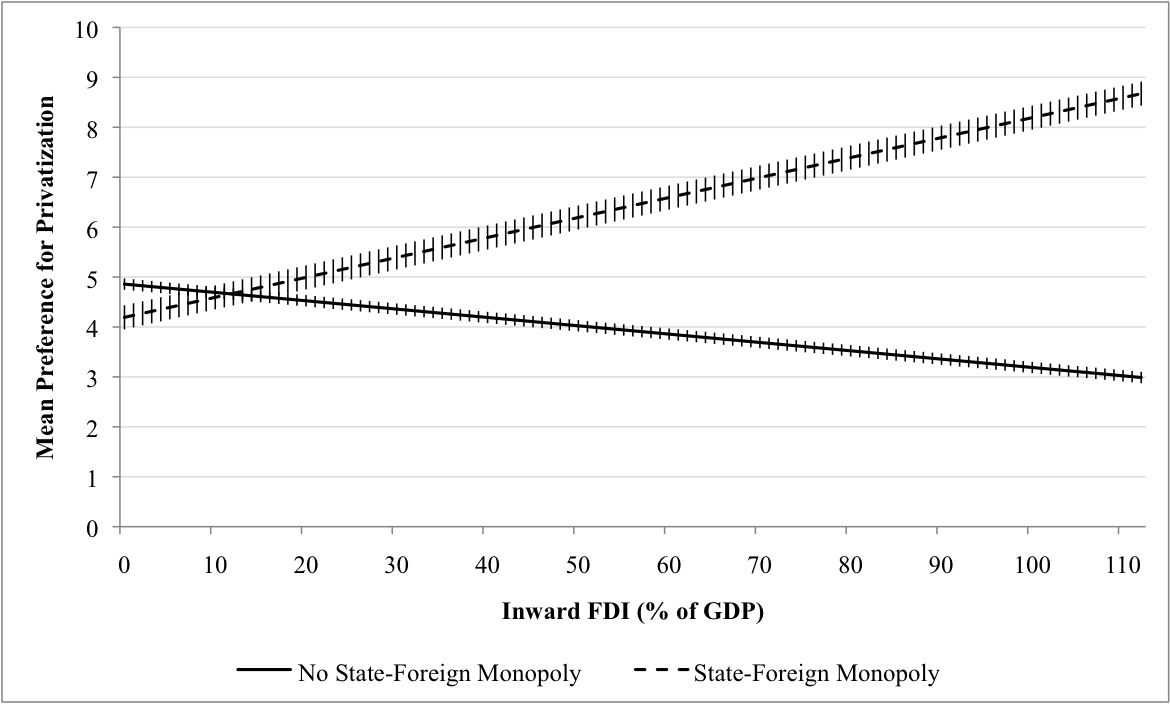
\includegraphics[scale=.75]{fdi.png}
\caption{{Inward FDI (\% of GDP) and Expected Preference for Privatization}}
\end{center}
\end{figure}

\begin{figure}[htbp]
\begin{center}
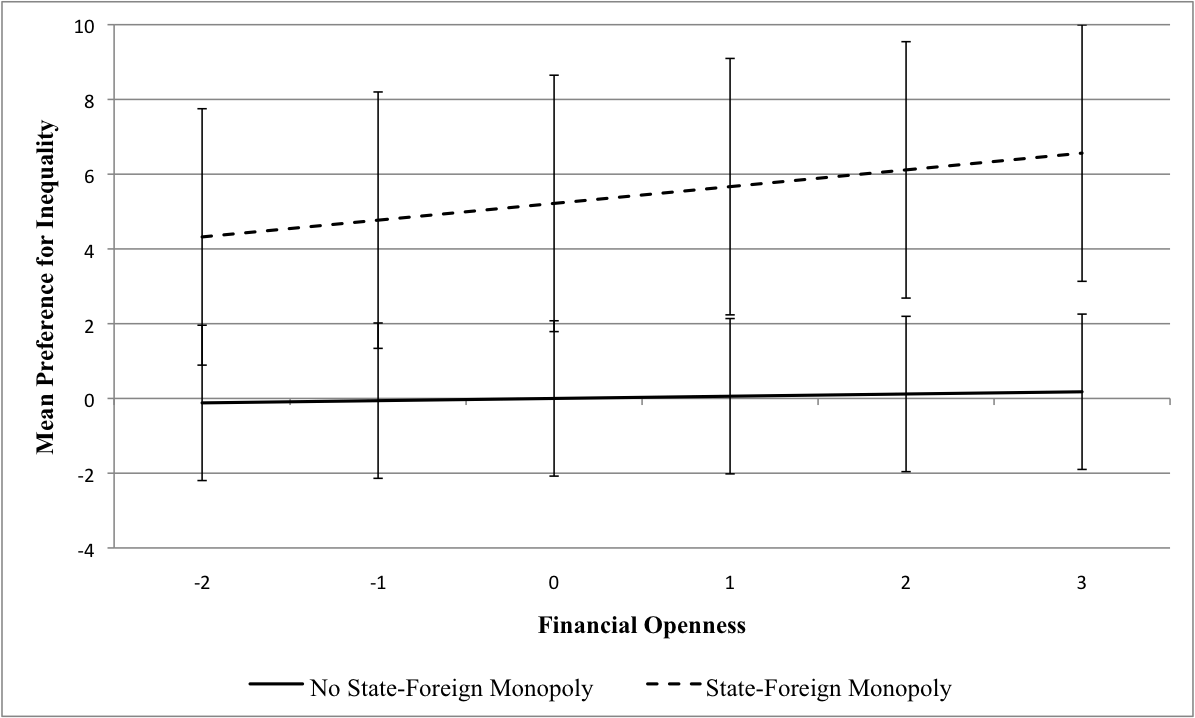
\includegraphics[scale=.75]{finopen.png}
\caption{{Financial Openness and Preference for Inequality}}
\end{center}
\end{figure}
Perhaps most interestingly, when the media is dominated by the state or foreign companies, the effect of globalization on attitudes is significant and as predicted in two cases. For instance, other things equal, people prefer less privatization as foreign direct investment enters their country; when there is a duopoly between the state and foreign companies, actors who have common biases against the costs of globalization, then foreign-direct investment flows increase the desire for privatization. We find the same reversal with respect to the tolerance of inequality under financial openness. Although capital mobility, other things equal, does not have a statistically significant effect on the demand for reducing inequality, when mediated by a state-foreign media duopoly capital mobility is associated with favorable views regarding inequality as an incentive. Interesting as these findings are, this evidence in support of Hypothesis 2 are only two cases out of a total of nine combinations of alternative measures. In six other interaction terms, there is no statistically significant result and in one the relationship ($tradeXduop$) runs counter to Hypothesis 2. At least within the sample, in five of the nine combinations the coefficient is larger than the non-interacted globalization measures, as predicted, with state-foreign domination of the media decreasing attitudes in support of goverment intervention.

	Trade is anomalous with respect to its non-interacted and interacted terms. Surpisingly, trade seems to correlate negatively with the demand for government intervention and positively when interacted with a state-foreign media duopoly.
	
	These findings require caution. It is well known that survey respondents are extremely sensitive to question wording. On the whole, these results are far from definitive proof that the link between global market exposure and demand for public support is significantly and consistently conditioned by media ownership. Neither is it definitive proof one way or the other regarding the micro-processes of the compensation thesis. But as a first interrogation of these links, the results are certainly sufficient to conclude that the assumptions of the compensation thesis require further investigation and should not be taken for granted as in the seminal works of the globalization-welfare literature. Second, although the results regarding the media as conditioning the reception of globalization are also mixed, there is at least modest evidence for this argument. For the same reasons these results should not be interpreted as conclusively disproving the compensation thesis, the mixed evidence regarding the media's conditional effect calls for more research on this hypothesis.
	 
	 The results of secondary regressions, with country fixed-effects, controls for pure and impure serial correlation, and disaggregated media ownership, are presented below. Woolridge's test for serial correlation in panel data show that very likely serial correlation is a problem in each case except for the models using attitudes toward inequality as the dependent variable (p = 0.0066 for attitudes toward privatization; p = 0.0347 for attitudes toward responsibility). In the first of the secondary regressions, we find evidence in favor of the compensation thesis (H1) and of media's conditioning effect (H2). Independently, FDI significantly decreases attitudes favorable toward privatization in two of three cases controlling for media ownership. Trade has a similar effect in only one case, when foreign ownership is controlled for. Financial openness never has the effect predicted by the compensation thesis. The interaction of FDI with media ownership is not significant when we consider foreign ownership alone, but it is significant in the hypothesized direction when we consider state ownership and the combined effects of foreign and state ownership. Conversely, the interaction of trade and media ownership is not significant with respect to state ownership, but it is significant with respect to foreign ownership and the combined measure.
\begin{table}[htdp]
\caption{Dependent Variable: Attitudes in Favor of Privatization}
\vspace{2em}
\begin{center}
{\small
\begin{tabular}{lccc} \hline
 & (1) & (2) & (3) \\
VARIABLES & Foreign & State & Foreign + State \\ \hline
\vspace{4pt} & \begin{footnotesize}\end{footnotesize} & \begin{footnotesize}\end{footnotesize} & \begin{footnotesize}\end{footnotesize} \\
fdi & -0.05 & -0.14* & -0.17* \\
\vspace{4pt} & \begin{footnotesize}(0.050)\end{footnotesize} & \begin{footnotesize}(0.058)\end{footnotesize} & \begin{footnotesize}(0.067)\end{footnotesize} \\
ttrade & -0.12*** & -0.07 & -0.12 \\
\vspace{4pt} & \begin{footnotesize}(0.034)\end{footnotesize} & \begin{footnotesize}(0.097)\end{footnotesize} & \begin{footnotesize}(0.099)\end{footnotesize} \\
finance & 0.06 & 0.46 & 0.94 \\
\vspace{4pt} & \begin{footnotesize}(0.549)\end{footnotesize} & \begin{footnotesize}(1.351)\end{footnotesize} & \begin{footnotesize}(1.158)\end{footnotesize} \\
percentforeign & -73.94*** &  &  \\
\vspace{4pt} & \begin{footnotesize}(21.927)\end{footnotesize} & \begin{footnotesize}\end{footnotesize} & \begin{footnotesize}\end{footnotesize} \\
fdiXforeign & 0.53 &  &  \\
\vspace{4pt} & \begin{footnotesize}(0.359)\end{footnotesize} & \begin{footnotesize}\end{footnotesize} & \begin{footnotesize}\end{footnotesize} \\
tradeXforeign & 0.89* &  &  \\
\vspace{4pt} & \begin{footnotesize}(0.364)\end{footnotesize} & \begin{footnotesize}\end{footnotesize} & \begin{footnotesize}\end{footnotesize} \\
financeXforeign & 1.97 &  &  \\
\vspace{4pt} & \begin{footnotesize}(3.217)\end{footnotesize} & \begin{footnotesize}\end{footnotesize} & \begin{footnotesize}\end{footnotesize} \\
percentstate &  & -31.32 &  \\
\vspace{4pt} & \begin{footnotesize}\end{footnotesize} & \begin{footnotesize}(20.004)\end{footnotesize} & \begin{footnotesize}\end{footnotesize} \\
fdiXstate &  & 0.79* &  \\
\vspace{4pt} & \begin{footnotesize}\end{footnotesize} & \begin{footnotesize}(0.330)\end{footnotesize} & \begin{footnotesize}\end{footnotesize} \\
tradeXstate &  & 0.26 &  \\
\vspace{4pt} & \begin{footnotesize}\end{footnotesize} & \begin{footnotesize}(0.250)\end{footnotesize} & \begin{footnotesize}\end{footnotesize} \\
financeXstate &  & 2.85 &  \\
\vspace{4pt} & \begin{footnotesize}\end{footnotesize} & \begin{footnotesize}(4.358)\end{footnotesize} & \begin{footnotesize}\end{footnotesize} \\
percentown &  &  & -39.64** \\
\vspace{4pt} & \begin{footnotesize}\end{footnotesize} & \begin{footnotesize}\end{footnotesize} & \begin{footnotesize}(14.150)\end{footnotesize} \\
fdiXfs &  &  & 0.66** \\
\vspace{4pt} & \begin{footnotesize}\end{footnotesize} & \begin{footnotesize}\end{footnotesize} & \begin{footnotesize}(0.232)\end{footnotesize} \\
tradeXfs &  &  & 0.40* \\
\vspace{4pt} & \begin{footnotesize}\end{footnotesize} & \begin{footnotesize}\end{footnotesize} & \begin{footnotesize}(0.201)\end{footnotesize} \\
financeXfs &  &  & -0.56 \\
\vspace{4pt} & \begin{footnotesize}\end{footnotesize} & \begin{footnotesize}\end{footnotesize} & \begin{footnotesize}(1.602)\end{footnotesize} \\
lagpriv & 0.80*** & 0.75*** & 0.70*** \\
\vspace{4pt} & \begin{footnotesize}(0.063)\end{footnotesize} & \begin{footnotesize}(0.134)\end{footnotesize} & \begin{footnotesize}(0.097)\end{footnotesize} \\
Constant & 15.47*** & 15.18 & 21.27** \\
 & \begin{footnotesize}(3.022)\end{footnotesize} & \begin{footnotesize}(9.043)\end{footnotesize} & \begin{footnotesize}(7.894)\end{footnotesize} \\
\vspace{4pt} & \begin{footnotesize}\end{footnotesize} & \begin{footnotesize}\end{footnotesize} & \begin{footnotesize}\end{footnotesize} \\
Observations & 30 & 30 & 30 \\
$R^2$ & 0.86 & 0.85 & 0.87 \\
Number of cntry & 10 & 10 & 10 \\
 $Rho$ & -.07 & -.19 & -.18 \\ \hline
\multicolumn{4}{c}{\begin{footnotesize} Standard errors in parentheses.\end{footnotesize}} \\
\multicolumn{4}{c}{\begin{footnotesize} *** p$<$0.001, ** p$<$0.01, * p$<$0.05\end{footnotesize}} \\
\multicolumn{4}{c}{\begin{footnotesize} Coefficients for country fixed-effects are not displayed. \end{footnotesize}} \\

\end{tabular}
}
\end{center}
\label{default}
\end{table}


\begin{table}[htdp]
\caption{Dependent Variable: Attitudes in Favor of Inequality}
\vspace{2em}
\begin{center}
{\small
\begin{tabular}{lccc} \hline
 & (1) & (2) & (3) \\
VARIABLES & Foreign & State & Foreign+State \\ \hline
\vspace{4pt} & \begin{footnotesize}\end{footnotesize} & \begin{footnotesize}\end{footnotesize} & \begin{footnotesize}\end{footnotesize} \\
fdi & -0.18 & -0.01 & -0.13 \\
\vspace{4pt} & \begin{footnotesize}(0.122)\end{footnotesize} & \begin{footnotesize}(0.108)\end{footnotesize} & \begin{footnotesize}(0.125)\end{footnotesize} \\
ttrade & 0.11 & 0.07 & 0.09 \\
\vspace{4pt} & \begin{footnotesize}(0.121)\end{footnotesize} & \begin{footnotesize}(0.073)\end{footnotesize} & \begin{footnotesize}(0.109)\end{footnotesize} \\
finance & 1.96** & 1.61* & 2.68*** \\
\vspace{4pt} & \begin{footnotesize}(0.634)\end{footnotesize} & \begin{footnotesize}(0.630)\end{footnotesize} & \begin{footnotesize}(0.659)\end{footnotesize} \\
percentforeign & 23.39 &  &  \\
\vspace{4pt} & \begin{footnotesize}(39.784)\end{footnotesize} & \begin{footnotesize}\end{footnotesize} & \begin{footnotesize}\end{footnotesize} \\
fdiXforeign & 0.38 &  &  \\
\vspace{4pt} & \begin{footnotesize}(0.672)\end{footnotesize} & \begin{footnotesize}\end{footnotesize} & \begin{footnotesize}\end{footnotesize} \\
tradeXforeign & -0.14 &  &  \\
\vspace{4pt} & \begin{footnotesize}(0.687)\end{footnotesize} & \begin{footnotesize}\end{footnotesize} & \begin{footnotesize}\end{footnotesize} \\
financeXforeign & -20.56*** &  &  \\
\vspace{4pt} & \begin{footnotesize}(5.998)\end{footnotesize} & \begin{footnotesize}\end{footnotesize} & \begin{footnotesize}\end{footnotesize} \\
percentstate &  & 52.32 &  \\
\vspace{4pt} & \begin{footnotesize}\end{footnotesize} & \begin{footnotesize}(29.819)\end{footnotesize} & \begin{footnotesize}\end{footnotesize} \\
fdiXstate &  & -1.28 &  \\
\vspace{4pt} & \begin{footnotesize}\end{footnotesize} & \begin{footnotesize}(0.852)\end{footnotesize} & \begin{footnotesize}\end{footnotesize} \\
tradeXstate &  & -0.47 &  \\
\vspace{4pt} & \begin{footnotesize}\end{footnotesize} & \begin{footnotesize}(0.351)\end{footnotesize} & \begin{footnotesize}\end{footnotesize} \\
financeXstate &  & -13.79** &  \\
\vspace{4pt} & \begin{footnotesize}\end{footnotesize} & \begin{footnotesize}(5.093)\end{footnotesize} & \begin{footnotesize}\end{footnotesize} \\
percentown &  &  & 10.59 \\
\vspace{4pt} & \begin{footnotesize}\end{footnotesize} & \begin{footnotesize}\end{footnotesize} & \begin{footnotesize}(16.050)\end{footnotesize} \\
fdiXfs &  &  & -0.08 \\
\vspace{4pt} & \begin{footnotesize}\end{footnotesize} & \begin{footnotesize}\end{footnotesize} & \begin{footnotesize}(0.406)\end{footnotesize} \\
tradeXfs &  &  & -0.12 \\
\vspace{4pt} & \begin{footnotesize}\end{footnotesize} & \begin{footnotesize}\end{footnotesize} & \begin{footnotesize}(0.294)\end{footnotesize} \\
financeXfs &  &  & -8.14*** \\
\vspace{4pt} & \begin{footnotesize}\end{footnotesize} & \begin{footnotesize}\end{footnotesize} & \begin{footnotesize}(1.276)\end{footnotesize} \\
lagineq & 0.19 & 0.03 & 0.08 \\
\vspace{4pt} & \begin{footnotesize}(0.208)\end{footnotesize} & \begin{footnotesize}(0.180)\end{footnotesize} & \begin{footnotesize}(0.184)\end{footnotesize} \\
Constant & 40.80*** & 49.30*** & 46.47*** \\
 & \begin{footnotesize}(11.870)\end{footnotesize} & \begin{footnotesize}(11.757)\end{footnotesize} & \begin{footnotesize}(11.794)\end{footnotesize} \\
\vspace{4pt} & \begin{footnotesize}\end{footnotesize} & \begin{footnotesize}\end{footnotesize} & \begin{footnotesize}\end{footnotesize} \\
Observations & 30 & 30 & 30 \\
$R^2$ & 0.58 & 0.37 & 0.37 \\
Number of cntry & 10 & 10 & 10 \\
 $Rho$ & -.15 & .12 & -.03 \\ \hline
\multicolumn{4}{c}{\begin{footnotesize} Standard errors in parentheses\end{footnotesize}} \\
\multicolumn{4}{c}{\begin{footnotesize} *** p$<$0.001, ** p$<$0.01, * p$<$0.05\end{footnotesize}} \\
\multicolumn{4}{c}{\begin{footnotesize} Coefficients for country fixed-effects are not displayed. \end{footnotesize}} \\
\end{tabular}
}
\end{center}
\label{default}
\end{table}



Results for attitudes toward inequality show no evidence in favor of either the compensation thesis or the media interaction hypothesis. It is possible that attitudes towards whether the government should intervene to lessen inequality reflect more than the demand for state intervention in general, more so than attitudes toward privatization.

When using measures of attitudes toward personal versus government responsibility as the dependent variable, we find evidence that FDI significantly decreases the attitude that people should be more responsible, but evidence that trade either has no significant effect or it increases the belief in personal responsibility in the case that we control for foreign media ownership. More interestingly, we find evidence that state ownership and foreign plus state ownership significantly condition the effect that FDI and trade have on attitudes toward who should be more responsible. Again, the effects are in the predicted direction, with state ownership reversing the effect of two globalization processes, from increasing the belief that the government should be more responsible to increasing beliefs that individuals should be more responsible instead.


\begin{table}[htdp]
\caption{Dependent Variable: Attitudes in Favor of Personal Responsibility}
\vspace{2em}
\begin{center}
{\small
\begin{tabular}{lccc} \hline
 & (1) & (2) & (3) \\
VARIABLES & Foreign & State & Foreign+State \\ \hline
\vspace{4pt} & \begin{footnotesize}\end{footnotesize} & \begin{footnotesize}\end{footnotesize} & \begin{footnotesize}\end{footnotesize} \\
fdi & -0.19* & -0.34*** & -0.22** \\
\vspace{4pt} & \begin{footnotesize}(0.087)\end{footnotesize} & \begin{footnotesize}(0.060)\end{footnotesize} & \begin{footnotesize}(0.082)\end{footnotesize} \\
ttrade & 0.21* & 0.12 & 0.08 \\
\vspace{4pt} & \begin{footnotesize}(0.095)\end{footnotesize} & \begin{footnotesize}(0.096)\end{footnotesize} & \begin{footnotesize}(0.122)\end{footnotesize} \\
finance & 0.91 & 2.82*** & 2.03* \\
\vspace{4pt} & \begin{footnotesize}(0.551)\end{footnotesize} & \begin{footnotesize}(0.573)\end{footnotesize} & \begin{footnotesize}(0.796)\end{footnotesize} \\
percentforeign & -37.50 &  &  \\
\vspace{4pt} & \begin{footnotesize}(36.474)\end{footnotesize} & \begin{footnotesize}\end{footnotesize} & \begin{footnotesize}\end{footnotesize} \\
fdiXforeign & 1.00 &  &  \\
\vspace{4pt} & \begin{footnotesize}(0.573)\end{footnotesize} & \begin{footnotesize}\end{footnotesize} & \begin{footnotesize}\end{footnotesize} \\
tradeXforeign & 0.17 &  &  \\
\vspace{4pt} & \begin{footnotesize}(0.654)\end{footnotesize} & \begin{footnotesize}\end{footnotesize} & \begin{footnotesize}\end{footnotesize} \\
financeXforeign & -4.16 &  &  \\
\vspace{4pt} & \begin{footnotesize}(4.048)\end{footnotesize} & \begin{footnotesize}\end{footnotesize} & \begin{footnotesize}\end{footnotesize} \\
percentstate &  & -101.88*** &  \\
\vspace{4pt} & \begin{footnotesize}\end{footnotesize} & \begin{footnotesize}(28.788)\end{footnotesize} & \begin{footnotesize}\end{footnotesize} \\
fdiXstate &  & 1.96** &  \\
\vspace{4pt} & \begin{footnotesize}\end{footnotesize} & \begin{footnotesize}(0.621)\end{footnotesize} & \begin{footnotesize}\end{footnotesize} \\
tradeXstate &  & 0.80** &  \\
\vspace{4pt} & \begin{footnotesize}\end{footnotesize} & \begin{footnotesize}(0.298)\end{footnotesize} & \begin{footnotesize}\end{footnotesize} \\
financeXstate &  & -9.90** &  \\
\vspace{4pt} & \begin{footnotesize}\end{footnotesize} & \begin{footnotesize}(3.775)\end{footnotesize} & \begin{footnotesize}\end{footnotesize} \\
percentown &  &  & -52.40** \\
\vspace{4pt} & \begin{footnotesize}\end{footnotesize} & \begin{footnotesize}\end{footnotesize} & \begin{footnotesize}(17.727)\end{footnotesize} \\
fdiXfs &  &  & 0.82** \\
\vspace{4pt} & \begin{footnotesize}\end{footnotesize} & \begin{footnotesize}\end{footnotesize} & \begin{footnotesize}(0.296)\end{footnotesize} \\
tradeXfs &  &  & 0.57* \\
\vspace{4pt} & \begin{footnotesize}\end{footnotesize} & \begin{footnotesize}\end{footnotesize} & \begin{footnotesize}(0.280)\end{footnotesize} \\
financeXfs &  &  & -4.58* \\
\vspace{4pt} & \begin{footnotesize}\end{footnotesize} & \begin{footnotesize}\end{footnotesize} & \begin{footnotesize}(2.096)\end{footnotesize} \\
lagresp & 0.71*** & 0.29 & 0.55*** \\
\vspace{4pt} & \begin{footnotesize}(0.142)\end{footnotesize} & \begin{footnotesize}(0.153)\end{footnotesize} & \begin{footnotesize}(0.105)\end{footnotesize} \\
Constant & 7.89 & 32.69*** & 21.10*** \\
 & \begin{footnotesize}(4.789)\end{footnotesize} & \begin{footnotesize}(9.112)\end{footnotesize} & \begin{footnotesize}(5.687)\end{footnotesize} \\
\vspace{4pt} & \begin{footnotesize}\end{footnotesize} & \begin{footnotesize}\end{footnotesize} & \begin{footnotesize}\end{footnotesize} \\
Observations & 30 & 30 & 30 \\
$R^2$ & 0.60 & 0.62 & 0.75 \\
Number of cntry & 10 & 10 & 10 \\
 $Rho$ & -.08 & -.01 & -.19 \\ \hline
\multicolumn{4}{c}{\begin{footnotesize} Standard errors in parentheses\end{footnotesize}} \\
\multicolumn{4}{c}{\begin{footnotesize} *** p$<$0.001, ** p$<$0.01, * p$<$0.05\end{footnotesize}} \\
\multicolumn{4}{c}{\begin{footnotesize} Coefficients for country fixed-effects are not displayed. \end{footnotesize}} \\
\end{tabular}
}
\end{center}
\label{default}
\end{table}

\pagebreak

\subsection{A Quantitative Analysis of Independent News LTD}
Reported below are the regression results analyzing the relationship between globalizing processes and mentions of globalization in 12 INL newspapers before and after their purchase by foreign-owned John Fairfax Holdings. The variable of interest is the first variable reported, the interaction term representing New Zealand trade filtered through Fairfax ownership. The significant and negatively signed coefficient suggests that under Fairfax, the papers' reportage of globalization was significantly less an increasing function of New Zealand trade than before Fairfax.

\pagebreak
\begin{center}
\begin{table}[htdp]
\caption{Multiple Regression with Panel-Corrected Standard Errors}
\vspace{2em}

\begin{center}
{\small
\begin{tabular}{lc} \hline
 &  \\
Independent Variables & Coefficient \\ \hline
\vspace{4pt} & \begin{footnotesize}\end{footnotesize} \\
tradeXfairfax & -110.45* \\
\vspace{4pt} & \begin{footnotesize}(43.945)\end{footnotesize} \\
nztrade & 135.36*** \\
\vspace{4pt} & \begin{footnotesize}(21.069)\end{footnotesize} \\
fairfax & 67.55** \\
\vspace{4pt} & \begin{footnotesize}(25.692)\end{footnotesize} \\
wtrade & -0.00 \\
\vspace{4pt} & \begin{footnotesize}(0.000)\end{footnotesize} \\
fdi & -13.98 \\
\vspace{4pt} & \begin{footnotesize}(16.475)\end{footnotesize} \\
thailand & -4.69** \\
\vspace{4pt} & \begin{footnotesize}(1.708)\end{footnotesize} \\
asean & 0.09 \\
\vspace{4pt} & \begin{footnotesize}(3.405)\end{footnotesize} \\
china & -2.30 \\
\vspace{4pt} & \begin{footnotesize}(2.661)\end{footnotesize} \\
singapore & -8.58*** \\
\vspace{4pt} & \begin{footnotesize}(1.970)\end{footnotesize} \\
lag & 0.25* \\
\vspace{4pt} & \begin{footnotesize}(2.258)\end{footnotesize} \\
Constant & -67.82*** \\
 & \begin{footnotesize}(12.599)\end{footnotesize} \\
\vspace{4pt} & \begin{footnotesize}\end{footnotesize} \\
Observations & 153 \\
Number of newspapers & 12 \\
$R^2$ & 0.86 \\
 Adj. $R^2$ & . \\ \hline
\multicolumn{2}{c}{\begin{footnotesize} Includes fixed effects by newspaper. \end{footnotesize}} \\
\multicolumn{2}{c}{\begin{footnotesize} *** p$<$0.001, ** p$<$0.01, * p$<$0.05\end{footnotesize}} \\
\end{tabular}
}
\end{center}

\label{default}
\end{table}
\end{center}

This is evidence in favor of the foreign-ownership part of Hypothesis 3, namely that the bias of foreign-ownership is likely to imply a functional disconnect between real-world, national economic integration in the global economy and reportage of globalization. Graphically, it is easy to observe that when one runs separate regressions for the years 1995-2003 and 2003-2009, the slope is significantly steeper and there is less standard error in the first period. The graph is only interesting descriptively because the confidence intervals are inflated by separating the data into two samples and running two separate regressions. The significance of the interaction term in the full model shows that the difference is significant. I argue that this is modest evidence in favor of the hypothesis that foreign-owned media outlets are likely to be biased toward globalization in a way that represents it in a way disconnected from the real, lived experiences of a particular national public.

\begin{center}
\begin{figure}[htbp]
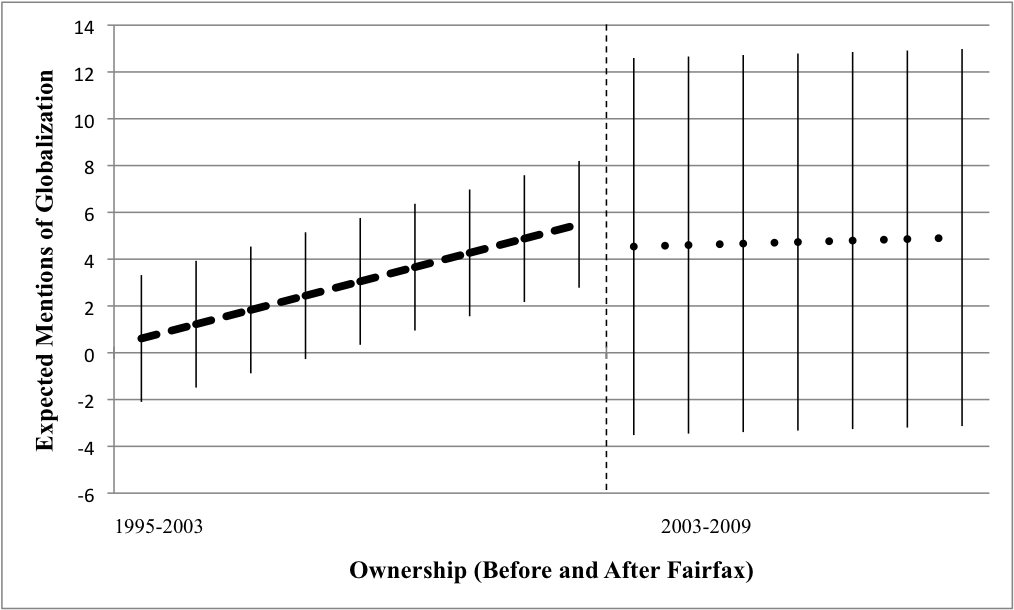
\includegraphics[scale=.85]{rdgraph.png}
\caption{{Discontinuous Regressions for Reportage of  Globalization and New Zealand Trade, 1995-2009
}}
\end{figure}
\end{center}

\subsection{A Qualitative Comparison of Media Representations}

To begin analysis of the actual social construction of globalization, consider the following table which summarizes total number of news stories reporting on two major FTAs signed by New Zealand in the past decade. Content analysis of newspaper reports in these time spans considered an article to be "negative/debatable" if it mentioned any viewpoint critical of globalization or if it mentioned that globalization is debated. Immediately, one notices that in the year leading up to an agreement, the year of an agreement, and the year after an agreement, news reports under Fairfax are relatively few, late, and uncritical.

\begin{center}
\begin{table}[htdp]
\caption{Comparison of TPSEP and NZSCEP Media Reports}
\vspace{2em}
\begin{center}
{\small
\begin{tabular}{lcccc} \hline
& $T_{-1}$ &  $T$ &  $T_{+1}$ & Total \\ \hline
& \begin{footnotesize}\end{footnotesize} & \begin{footnotesize}\end{footnotesize} & \begin{footnotesize}\end{footnotesize} \\
\bf{TPSEP} & & & &\\
Yearly Total & 0 & 0 & 3 & 3\\
\# Negative/Debatable & 0 & 0 & 0 & 0 \vspace{4pt} \\
\bf{NZSCEP} & & & & \\
Yearly Total & 0 & 7 & 1 & 8\\
\# Negative/Debatable & 0 & 6 & 1 & 7 \vspace{10pt}\\
\end{tabular}
}
\end{center}
\label{default}
\end{table}
\end{center}


More specifically, content analysis reveals the following distinct pattern of representation. After 2003, one finds in the pages of INL newspapers a \emph{naturalization} of globalization. In the reports on the 2001 NZSCEP, globalization is a political phenomenon with proponents and critics debating the issue. For instance, six of the reports are ``Day in the House" articles reporting that the legislature was actively reviewing and debating the proposed NZSCEP. The NZSCEP is an uncertain prospect with costs and benefits, as well as proponents (Labour and National parties) and opponents (Alliance and Green parties) (Evening Post, Nov. 16, 2000). In contrast, after 2006, in the three stories reporting on the TPSEP, it is striking that in each case, the defining problematic which makes the story newsworthy is that New Zealand is suffering in one way or another from \emph{not enough} free trade. (Dominion Post 2006; Timaru Herald 2006; The Press 2006). A representative example is the second sentence in the 2006 article from \emph{The Press}, which is supposed to capture the interest of the reader with "growing fears New Zealand may be losing out in the race to clinch bilateral deals to remove trade barriers such as tariffs and quotas." Noticeably, Lexis-Nexis finds zero "Day in the House" articles such as those that represented the NZSCEP as a legislative debate. In 2006, globalization becomes a given, something that \emph{happened}. Thus, a strikingly noticeable qualitative difference in the social construction of globalization emerges after a shift toward foreign ownership: globalizing free-trade agreements that were previously represented as contentious, debatable, prospective political issues become already decided, hardly arguable, given or naturalized facts.


\section{Conclusion}

To conclude, I find mixed but suggestive evidence, from three levels of analysis, that media ownership significantly conditions the political response of mass publics toward globalization. The main quantitative analysis reveal that the assumptions of the compensation thesis are problematic: in relatively few of the different model specifications examining different measures of globalization and different attitudes toward government intervention was there significant evidence that people demand government intervention to compensate for exposure to global free trade. In relatively few cases was the sign of the coefficient even as predicted by this thesis. The main findings of interest, and the main potential contribution of this paper, relate to the effect of media ownership in mediating the political response to exposure to global free trade. Although findings were not consistent and were very sensitive to model specification, more than half of the total cross-national models showed that either foreign or state ownership significantly dampened or reversed the effect of some globalization process on some attitude toward the demand for state intervention. Given the shortcomings of the data, I interpret the sum of the findings as a promising warrant for more research on this question. In short, the findings problematize accepted wisdom and provide a suggestive first cut at a fairly new, fairly bold hypothesis. The within-case quantitative and qualitative evidence further suggest that media ownership significantly determines bias in the social construction of globalization.


\section{Appendix}

\begin{table}[htdp]
\caption{Appendix: Countries in Main Quantitative Analysis}
\begin{center}
\vspace{2em}
\begin{tabular}{ccc}
Albania & Algeria & Argentina \\ \\
Armenia & Australia & Azerbaijian \\ \\
Bangladesh & Belarus & Belgium \\ \\
Bosnia Herzegovina & Brazil & Bulgaria \\ \\
Canada & Chile & China \\ \\
Colombia & Croatia & Czech Republic \\ \\
Dominican Republic & Egypt & El Salvador \\ \\
Estonia & Finland & France \\ \\
Georgia & Ghana & Guatemala \\ \\
Hungary & Iceland & India \\ \\
Ireland & Italy & Japan \\ \\
Korea & Mexico & Netherlands \\ \\
New Zealand & Norway & Poland \\ \\
Slovenia & Spain & Sweden \\ \\
Switzerland & Turkey & United Kingdom \\ \\
United States & Venezuela \\ \\


\end{tabular}
\end{center}
\label{default}
\end{table}%


\bibliographystyle{apsr2006}

\bibliography{mybib}

\end{document}